In this part, we discuss the presence of non-negative equilibrium points for our system. Initially, we consider the function $f(n) = 1 - \frac{\psi(n)}{\phi(n)}$. It is assumed that $f(0)>0$, with $f$ increasing for relatively small values of $n$ and decreasing as $n$ becomes significantly large. These characteristics of the function mirror the biological phenomenon where a low viral load encourages the growth of immune
cells, whereas a high infection level reduces cell proliferation and augments cell mortality. The function $f$ presents two scenarios:
(i) it can stay positive across all values of $n$, or (ii) alternatively, it may turn negative when $n$ reaches a certain threshold. here we focus on the latter scenario.

The equilibrium points coincide with the solutions of :

\begin{equation}
	\begin{cases}
		 \mu(1 - a)  = 0 \\
		 \eta_s(1 - n)s - \alpha as - \beta \frac{sr}{n} - \gamma sp = 0 \\
		 \eta_r(1 - n)r + \beta \frac{sr}{n} - \gamma rp = 0 \\
		 \phi(n)p(f(n) -p ) = 0 
	\end{cases}
\end{equation}

which is equivalent to:

\begin{equation}
	\begin{cases}
		a = 1 \\
		s = 0 \quad \text{or} \quad \eta_s(1-n) - \alpha - \beta\frac{r}{n} -\gamma p =0 \\
		r = 0 \quad \text{or} \quad \eta_r(1-n) + \beta\frac{s}{n} -\gamma p =0 \\
		p = 0 \quad \text{or} \quad p = f(n) \\
	\end{cases}
\end{equation}

\begin{itemize}
	\item Case 1: \(r = s = p = 0\)
	
	We have the equilibrium \( E_0 (1,0,0,0)   \).
	\item Case 2:  \( r = s = 0 \ , \ p \neq 0 \)
	
	We obtain the equilibrium  \(E_1 (1,0,0,f(0)) \).
	\item Case 3:   \( s = p = 0 \ , \ r \neq 0 \)
	
	The equilibrium state is denoted as \(E_2 (1,0,1,0) \).
	\item Case 4: \( s = 0 \ , \ r \neq 0 \ , \ p \neq 0 \) 
	
	In this case, we have $r = \lambda_+$ and $p = f(\lambda_+)$ with $\lambda_+$ being the solution of the following equation: 
	
	\begin{equation}
		f(r) = \eta_r \frac{1 - r}{\gamma}
	\end{equation}

	$\lambda_+$ is identified at the points where the function $f$ intersects with the line $y= \eta_r \frac{1 - r}{\gamma}$. Therefor, if $f(0)< \frac{\eta_r}{\gamma} $ we will have a unique solution $0 < \lambda_+ < 1$ that satisfies our equation.
	
	\begin{figure}[h!]
		\centering
		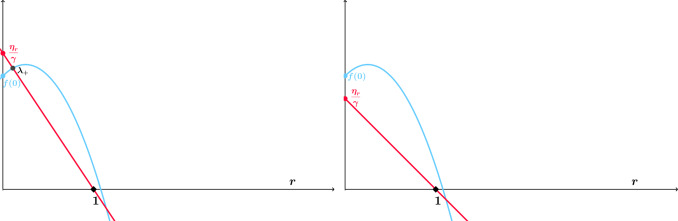
\includegraphics[width=0.7\textwidth]{1-s2.0-S1007570424005975-gr3.jpg}
		\caption{\(f\) and \(\lambda_+\)}
	\end{figure}
	
	\item Case 5:  \(s \neq 0 \ , \ r = 0 \ , \ p = 0 \)
	
	Here, we have the equilibrium $E_3(1,1-\frac{\alpha}{\eta_s},0,0)$ which exists if $\alpha<\eta_s$.
	
	\newpage
	\item Case 6:  \(s \neq 0 \ , \ r = 0 \ , \ p \neq 0 \)
	
	In this scenario, $s=\lambda_-$ and $p = f(\lambda_-)$, where $0 < \lambda_- < 1$ is the unique solution of this equation:
	\begin{equation}
		f(s) = \frac{\eta_s- \alpha}{\gamma} - \frac{\eta_s}{\gamma}s
	\end{equation}
	which exists for $f(0) < \frac{\eta_s- \alpha}{\gamma}$.
	
	\begin{figure}[h!]
		\centering
		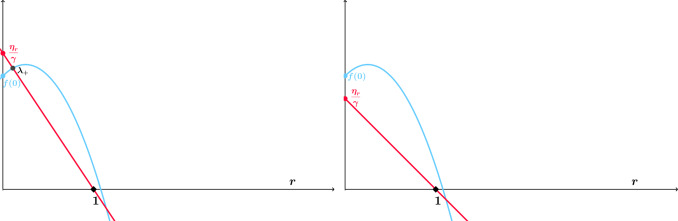
\includegraphics[width=0.7\textwidth]{1-s2.0-S1007570424005975-gr3.jpg}
		\caption{\(f\) and \(\lambda_-\)}
	\end{figure}

	

	\item Case 7:   \(s \neq 0 \ , \ r \neq 0 \ , \ p \neq 0 \)
	In this case, we obtain $n_* = s + r = 1 - \frac{\alpha + \beta}{\eta_s - \eta_r}$.
	
	This value of $n_*$ is positive under the condition that $\alpha + \beta + \eta_r < \eta_s$, hence, we have $p_* = f(n_*)$. Furthermore, the equations for $s_*$ and $r_*$ are given by:
	$$s_* = \frac{n_*}{\beta}\left( \gamma f(n_*) - \eta_r \frac{\alpha + \beta}{\eta_s - \eta_r} \right)$$
	$$r_* = \frac{n_*}{\beta}\left( \eta_s \frac{\alpha + \beta}{\eta_s - \eta_r} - \alpha - \gamma f(n_*) \right)$$
	and these values are positive under the condition
	$$\eta_r \frac{\alpha + \beta}{\eta_s - \eta_r} < \gamma f(n_*) < \frac{\alpha \eta_r + \beta \eta_s}{\eta_s - \eta_r}.$$
	
\end{itemize}


	